\documentclass{summarysheet}

\begin{document}


\maketitle{1}{Charge and Coulomb's Law}


\begin{multicols}{2}

\begin{topicbox}{What is charge?}

\begin{multicols}{2}

\noindent Charge is a property of electrons, which have negative charge, and protons, which have positive charge.
\begin{itemize}
\item All charged objects have either an excess of electrons or an excess of protons. Neutral objects have equal numbers of each.
\item Charges exert long-range forces between them: attractive for opposite charges, repulsive for like charges.
\end{itemize}

\vspace{1in}

\begin{center}
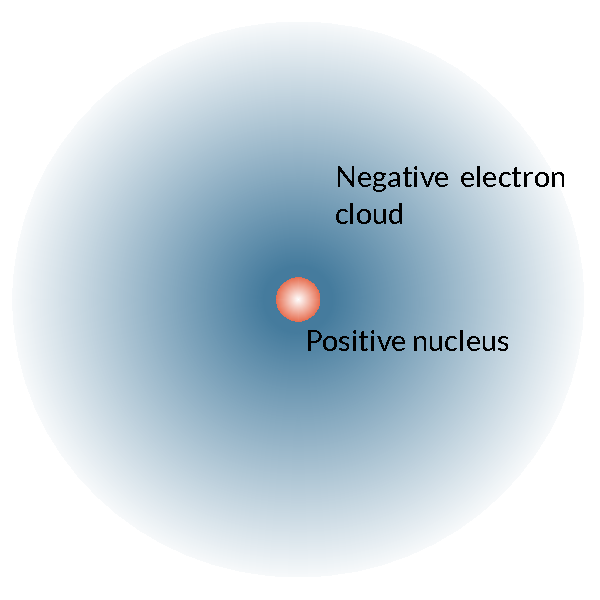
\includegraphics[scale=0.45]{fig_atom.pdf}
\end{center}


\end{multicols}

\begin{itemize}
\item Charge is quantized -- it always comes in amounts of $e$, called the elementary charge: $e = 1.60 \times 10^{-19}$ C.
\item Charge is always conserved.
\end{itemize}

\begin{center}
\begin{teqbox}
\begin{tabular}{ll}
\textbf{Proton} & \textbf{Electron} \\
Mass: $1.67 \times 10^{-27}$ kg & Mass: $9.11 \times 10^{-31}$ kg \\
Charge: $+e = +1.60 \times 10^{-19}$ C & Charge: $-e = -1.60 \times 10^{-19}$ C
\end{tabular}
\end{teqbox}
\end{center}

\end{topicbox}



\begin{topicbox}{MODEL: Point Charges}


\noindent Many objects that have excess positive or negative charge can be modelled as point particles -- their size and shape can be neglected, and we can think of all excess charge as being concentrated at a specific point.

\begin{multicols}{2}
Good examples of point charges are electrons and protons, atomic or molecular ions, and even much larger objects such as photocopier toner beads.
\begin{center}
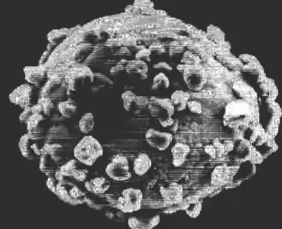
\includegraphics[scale=0.2]{fig_toner.png}
\end{center}
\end{multicols}

\end{topicbox}






\begin{topicbox}{Coulomb's Law}

\noindent Two point charges $q_1$ and $q_2$, a distance $r$ apart, exert forces on each other of magnitude
\[
F_\text{1 on 2} = F_\text{2 on 1} = \frac{1}{4\pi \epsilon_0} \frac{|q_1| |q_2|}{r^2}.
\]
The forces are directed along a line joining the two point charges, either repulsive for like charges or attractive for opposite charges.
\begin{center}
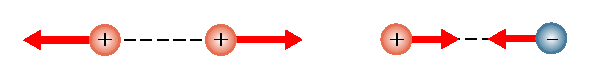
\includegraphics[scale=0.65]{fig_coulomb.pdf}
\end{center}

\begin{teqbox}
\noindent \textbf{Constants}

\noindent Permittivity constant: $\epsilon_0 = 8.85 \times 10^{-12}$ C$^2$/Nm$^2$.

\noindent Electrostatic constant: $K = \frac{1}{4\pi \epsilon_0} = 8.99 \times 10^{9}$ Nm$^2$/C$^2$.
\end{teqbox}

\end{topicbox}


\begin{topicbox}{Conductors and Insulators}

\noindent \textbf{Insulators}:  All electrons are tightly bound to their atoms.  Charges are fixed in place.

\noindent \textbf{Conductors}:  Valence electrons form a ``sea of electrons.''  Charges can move easily.  Any excess charge in an isolated conductor is located on the surface.

Both insulators and conductors can be \emph{charged}.

\end{topicbox}


\begin{topicbox}{Polarization}

\noindent Charge separation can easily occur in conductors, leading to \emph{polarization}: a slight separation of the positive and negative charges in a neutral object.

Polarization can also occur in insulators since each atom can become polarized, with a net overall polarization throughout the object.

Polarization can lead to an attractive polarization force between a charged object and a neutral object.

\begin{center}
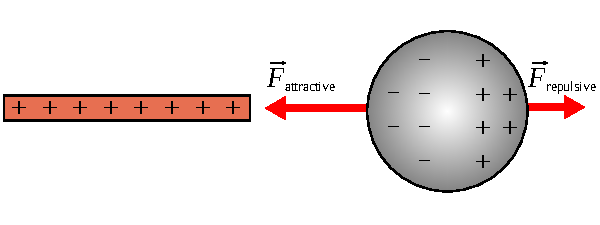
\includegraphics[scale=0.65]{fig_polarization.pdf}
\end{center}

\end{topicbox}






%\end{multicols}

\begin{topicbox}{Applying Coulomb's Law}

%\begin{multicols}{2}

\noindent When multiple point charges are present, use the \emph{principle of superposition} to find the net force on point charge 1:

\[
\vec{F}_\text{1,net} =  \vec{F}_\text{2 on 1} + \vec{F}_\text{3 on 1} + \vec{F}_\text{4 on 1} + \cdots
\]
For example, if there are three point charges arranged as shown below, you would add the forces due to charges $q_2$ and $q_3$ as vectors to find the net force on $q_1$.


\begin{center}
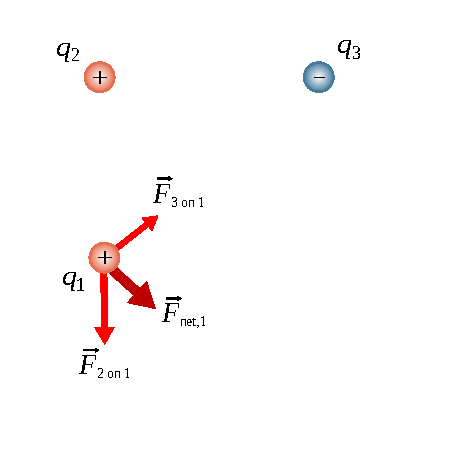
\includegraphics[scale=0.7]{fig_superposition.pdf}
\end{center}


\end{topicbox}


\end{multicols}


\makebanner{Electricity and Magnetism}

\end{document}



